\documentclass[a4paper,
oneside,
11pt,
abstracton,
% parskip, % add space between paragraphs
headsepline, % get a line under the header
]{scrreprt} %


\usepackage[utf8]{inputenc} % Required for inputting international characters

\usepackage[english, ngerman]{babel}

\usepackage[default]{lato}
\usepackage[T1]{fontenc}

\usepackage[bottom=30mm]{geometry} %Seitenränder
\usepackage[pdfborder={ 0 0 0 }, breaklinks, backref]{hyperref}

% ----------------------------------------------------------------


\usepackage[babel, german=swiss]{csquotes} % Required to generate language-dependent quotes in the bibliography

\usepackage{titleref}
\usepackage{cite}

\usepackage{wrapfig}
\usepackage{graphicx}
\graphicspath{{images/}}

\usepackage[table,xcdraw,dvipsnames]{xcolor}
\usepackage{float} % table float
\usepackage{booktabs} % need for table toprule etc

\usepackage{enumitem}
\linespread {1.25}\selectfont

% ------------------------------------------------------------

\addto\captionsngerman{\renewcommand{\abstractname}{Abstract}}

%------------------------------------------------

\usepackage{textcomp} % Fix warning with missing font shapes

%------------------------------------------------

\usepackage{xspace} % To get the spacing after macros right

%------------------------------------------------

\usepackage{mparhack} % To get marginpar right


%------------------------------------------------

\usepackage{scrhack} % Fix warnings when using KOMA with listings package

%------------------------------------------------

\usepackage{xspace} % setzt Leerzeichen, wenn welche hingehören

% --------------------------------------------

\usepackage[
nonumberlist,   %keine Seitenzahlen anzeigen
nopostdot,      %keine Punkte am Ende
acronym,       %ein Abkürzungsverzeichnis erstellen
toc]
{glossaries}
\makeglossaries
%Glossar-Befehle anschalten
\newglossaryentry{kollaborativ}{
    name={kollaborativ},
    description={ gemeinschaftlich}
}

% %%% define the acronym and use the see= option
% \newglossaryentry{C2X}{type=\acronymtype, name={C2X}, description={Car-to-X oder Vehicle-to-X}, first={Car-to-X (C2X)\glsadd{C2Xg}}, see=[Glossary:]{C2Xg}}
% \newglossaryentry{C2Ig}{
%     name={C2I},
%     description={ direkter, drahtloser Datenaustausch zwischen Fahrzeugen jeglicher Art und infrastrukturellen Einrichtungen wie Funkbaken und Lichtsignalanlagen auf Basis von \gls{WLAN}, Bluetooth oder \gls{DSRC}}
% }

\newglossaryentry{Netzwerklatenz}{
    name={Netzwerklatenz},
    description={ Die Wartezeit, die im Netzwerk verbraucht wird bevor eine Kommunikation beginnen kann, wird als Netzwerklatenz oder nur Latenz bezeichnet}
}

\newacronym{LWW}{LWW}{Last-Write-Wins}
\newacronym{CRDT}{CRDT}{Conflict-free replicated data type}
\newacronym{OT}{OT}{Operational Transformation}
%
\newacronym{API}{API}{Application Programming Interface}
\newacronym{App}{App}{Applikation}
\newacronym{JSON}{JSON}{JavaScript Object Notation}
\newacronym{PDF}{PDF}{Portable Document Format}
\newacronym{WLAN}{WLAN}{Wireless Local Area Network}
\newacronym{VM}{VM}{Virtual Machine}
\newacronym{XML}{XML}{Extensible Markup Language}
\newacronym{SQL}{SQL}{Structured Query Language}
\newacronym{UI}{UI}{User Interface}



% ---------------------------------------------------


\definecolor{lightgray}{gray}{0.95}
\definecolor{rulegray}{gray}{0.8}

\addtokomafont{chapter}{ \scshape \mdseries}
\addtokomafont{section}{\huge \scshape \mdseries \color{darkgray}}
\addtokomafont{subsection}{\LARGE \scshape \mdseries \color{gray}}
\addtokomafont{subsubsection}{\large \scshape \mdseries}
\setlength{\parindent}{0pt}  % keine Einrückungen nach Absätzen

\addto\captionsngerman{\renewcommand{\abstractname}{Abstract}}


\newcommand{\grayRule}{
   \textcolor{rulegray}{\rule{35em}{0.4pt}}
}


% ----------------------------------------------------

\usepackage{listings}
\lstdefinelanguage{JSON}{
	morestring=[b]",
	stringstyle=\color{purple},
    literate=
     *{0}{{{\color{violet}0}}}{1}
      {1}{{{\color{violet}1}}}{1}
      {2}{{{\color{violet}2}}}{1}
      {3}{{{\color{violet}3}}}{1}
      {4}{{{\color{violet}4}}}{1}
      {5}{{{\color{violet}5}}}{1}
      {6}{{{\color{violet}6}}}{1}
      {7}{{{\color{violet}7}}}{1}
      {8}{{{\color{violet}8}}}{1}
      {9}{{{\color{violet}9}}}{1}
      {false}{{{\color{violet}false}}}{1}
      {true}{{{\color{violet}true}}}{1}
      {:}{{{\color{blue}{:}}}}{1}
      {,}{{{\color{blue}{,}}}}{1}
      {\{}{{{\color{blue}{\{}}}}{1}
      {\}}{{{\color{blue}{\}}}}}{1}
      {[}{{{\color{blue}{[}}}}{1}
      {]}{{{\color{blue}{]}}}}{1},     ,
}
\lstset{
   captionpos=b,
   basicstyle=\scriptsize\ttfamily,
   keywordstyle=\bfseries\ttfamily\color{violet},
   stringstyle=\color{purple}\ttfamily,
   commentstyle=\color{OliveGreen}\ttfamily,
   backgroundcolor=\color{lightgray},
   emph={square},
   emphstyle=\color{blue}\texttt,
   emph={[2]root,base},
   emphstyle={[2]\color{yac}\texttt},
   showstringspaces=false,
   flexiblecolumns=false,
   tabsize=4,
   numbers=left,
   numberstyle=\tiny,
   numberblanklines=false,
   stepnumber=1,
   numbersep=5pt,
   xleftmargin=15pt
 }


%\addbibresource[label=ownpubs]{appendices/literatur.bib}

\begin{document}
\setlist{noitemsep}  %% verringert Zeilenabstand bei aufzaehlungen
\pagestyle{empty}

\begin{titlepage}

%\newcommand{\HRule}{\rule{\linewidth}{0.5mm}} % Defines a new command for the horizontal lines, change thickness here

\center % Center everything on the page


\begin{center}

\includegraphics[width=0.8\textwidth]{beuth}  \\[2cm]
\end{center}

\begin{Large}
Masterarbeit
\end{Large}\\[0.4cm]
\LARGE{Medieninformatik}\\
\large{Fachbereich VI -- Informatik und Medien}\\[0.5cm]


% \rule{length}{thickness}"
\rule{\textwidth}{0.4pt}\\[1cm] % Thin horizontal line
{\LARGE Untersuchung der Konfliktmanagementstrategien verschiedener offlinefähiger Systeme}\\[\baselineskip]

\rule{\textwidth}{0.4pt}\\[1cm]% Thin horizontal line

{\Large Berlin, den \today{}} %\\[6cm]
\vfill


\begin{minipage}{0.49\textwidth}
\begin{flushleft} \large
\emph{Autorin:}\\
Jacoba \textsc{Brandner} \\
\emph{Matrikelnummer:}\\
833753
\end{flushleft}
\end{minipage}
~
\begin{minipage}{0.49\textwidth}
\begin{flushright} \large
\emph{Betreuer:} \\
Herr Prof. Dr. Hartmut \textsc{Schirmacher} \\
\emph{Gutachter:} \\
Herr Prof. Dr. John \textsc{Doe} \\
\end{flushright}
\end{minipage}


\vfill % Fill the rest of the page with whitespace
\end{titlepage}

\begingroup
\let\titlepage\par
\let\endtitlepage
\let
\selectlanguage{ngerman}
\begin{abstract}
In dieser Arbeit wird eine Anwendung entwickelt, die ...\\
Hierzu wird analysiert welche Studien, Projekte oder Anwendungen es zu diesem Thema bereits gibt. Es wird diskutiert,.... Technischen und physikalischen Grundlagen erklärt. Hierb werden Definitionen und Entwicklungswerkzeuge beschrieben und ein Überblick über mögliche Einsatzgebiete gegeben. Für das Verständnis der Umsetzung ist die Klärung der ... erforderlich.\\
Die Konzipierung und Implementierung des exemplarischen Prototyps bilden den Kern dieser Arbeit, wobei dieser Prototyp in Architektur, Funktionalität und Design erläutert und schließlich in mehreren Testreihen evaluiert wird.
\end{abstract}
\selectlanguage{english}
\begin{abstract}
This work includes the development of an application  ...\\
Therefore it is analyzed which researches, projects and applications do already exist. It is going to be discussed ... technical base ... At this point definitions and developing tools are described and an overview of potential domains is given.\\
For comprehension the purification of the theoretical basis of the computation is necessary.\\
The conception and implementation of the showcase prototype is the core of this work. This is exemplified in architecture, functionality and design and finally evaluated in several test series.
\end{abstract}
\endgroup


\renewcommand{\contentsname}{Inhalt} %Inhaltsverzeichnistitel = Inhalt
\tableofcontents
\cleardoublepage
\pagestyle{headings} %Ab hier die Kopf-/Fusszeilen.
%\hyphenation{JavaScript} %trennt JavaScript nie


\chapter{\label{chap:einleitung}Einführung}
\begin{quote}
  We live in a disconnected \& battery powered world, but our technology and best practices are a leftover from the always connected \& steadily powered past.
  \cite{offlinefirst}
\end{quote}

\section{Motivation}
%\clearpage
\section{Zielstellung}


\chapter{\label{chap:grundlagen}Grundlagen}
Was bedeutet offlinefähig?\\\\
\textcolor{gray}{Software, mit der ein freigegebenes Dokument zusammen mit anderen über das Internet bearbeitet werden kann, kann überaus wertvoll sein wenn man beispielsweise in einem Team arbeitet. Heutzutage gibt es viele webbasierte Software für simultanes kollaboratives Editieren \textit{(Textdokumente, Tabellenkalkulationen, Präsentationen, Quellcode)}. Im Kapitel \ref{chap:state} werden Produkte und Frameworks vorgestellt, mit deren Hilfe man solche Software erstellen kann.\\
  Lassen Sie uns einen Moment nehmen, um genauer zu definieren, was wir unter dem Begriff kollaboratives Echtzeit-Editieren verstehen.
Wir möchten, dass mehrere Personen, die an verschiedenen Computern arbeiten, jederzeit Änderungen an einem auf einem Server gehosteten Dokument vornehmen können. Diese Änderungen werden sofort mit den anderen KollegInnen synchronisiert. Kein Client sollte vor einer Änderung mit dem Server oder einem anderen Client kommunizieren müssen. Insbesondere ist es nicht erforderlich, eine Sperre vom Server zu erhalten um ein Dokument zu bearbeiten und gleichzeitige Editierungen können auftreten. Nachdem alle Änderungen synchronisiert wurden, sollte jeder Client das exakt gleiche Dokument sehen.}
%
% Konflikte [Jan]
%
\section{\label{sec:conflict}Konflikte}
Verteilte Systeme: Das ist ein mächtiger Begriff für viele Ideen und Konzepten, aber es läuft in der Regel darauf hinaus: Da sind zwei oder mehr Computer, die durch ein Netzwerk verbunden sind und es wird versucht, dass einige der Daten auf beiden Computern gleich aussehen. ==> Ein System das zuverlässig über ein Netzwerk funktioniert.\\
Zwei Geräte, ein Server, über Netzwerk verbunden.\\\\
Spezielle Eigenschaft von Netzwerken: Verbindung kann jederzeit abbrechen:
Acht Irrtümer der verteilten Datenverarbeitung:
% \begin{enumerate}
%   \item Das Netzwerk ist zuverlässig
%   \item Die \gls{Latenz}zeit ist gleich null
%   \item Die Bandbreite ist unendlich
%   \item Das Netzwerk ist (informations)sicher
%   \item Die Netzwerkstruktur wird sich nicht ändern
%   \item Es gibt eineN AdministratorIn
%   \item Die Datentransportkosten sind gleich null
%   \item Das Netzwerk ist homogen
% \end{enumerate}
\begin{description}[leftmargin=0.5cm,style=nextline]
  \item[1. Das Netzwerk ist zuverlässig] ~ Der Strom kann ausfallen oder Glasfaserkabel können kaputt sein --- Das Netzwerk ist nicht zuverlässig.
 \item[2. Die \gls{Latenz} ist gleich null] ~ Glasfaserkabel werden durch Mikrowellen (oder andere Technologien) ersetzt um Millisekunden an Zeit zu sparen. Das würde nicht passieren, wäre die \gls{Latenz} bei null. Es dauert nun mal eine gewisse Zeit(ms) wenn ein Signal eine (geografisch)weite Strecke zurücklegen muss --- Die Latenz ist nicht gleich null.
 \item[3. Die \gls{Bandbreite} ist unendlich] ~ Daten können nicht schneller fließen als die Komponenten die sie verarbeiten (\gls{Middleware}, Datenbank \ldots) --- Die Bandbreite ist nicht unendlich.
 \item[4. Das Netzwerk ist sicher] ~ Der \sc{Heartbeat-bug}\footnote{\url{http://heartbleed.com/} -- Zugriff: 07.04.2018}, der im Jahr 2014 behoben wurde und die Sicherheitslücke im ICE-\gls{WLAN} im Jahr 2016\footnote{\url{https://netzpolitik.org/2016/datenschutz-im-zug-deutsche-bahn-will-sicherheitsluecke-in-neuem-ice-wlan-schliessen/} -- Zugriff: 07.04.2018} sind nur zwei Beispiele die zeigen, dass das Netzwerk nicht sicher ist.
 \item[5. Die Netzwerkstruktur wird sich nicht ändern] ~ Eine Datenbank kann beispielsweise über mehrere Server verteilt sein, die (teilweise) voneinander abhängig sind. Ein Server mit Abhängigkeiten kann ausfallen, es kann eine Aktualisierung für einen anderen Server geben --- die Struktur ändert sich.
 \item[5. Die Netzwerkstruktur wird sich nicht ändern] ~ Eine Datenbank kann beispielsweise über mehrere Server verteilt sein, die (teilweise) voneinander abhängig sind. Ein Server mit Abhängigkeiten kann ausfallen, es kann eine Aktualisierung für einen anderen Server geben --- die Struktur ändert sich.
 \item[6. Es gibt eineN AdministratorIn] ~ Es kann beliebig viele AdministratorInnen geben.
 \item[7. Die Datentransportkosten sind gleich null] ~ Netflix bezahlte anfang 2014 diversen InternetanbieterInnen dafür, dass Netflix KundInnen bevorzugten Internetzugang haben.
 \item[8. Das Netzwerk ist homogen] ~ Es gibt verschiedene Arten von Netzwer: 3G, 4G, LTE, WiFi. Wird beeinflusst durch Hardware (Smartphone, Tablet, PC, Laptop, Router \ldots)~\cite{fallacies}
\end{description}
\sub{\gls{CAP} Theorem?}
%
% Offline-First
%
\section{Offline First}
1. Separate Apps from Data\\
2. Deliver App Code (and make it cachable) {appcache \& ServiceWorkers}\\
3. Save Data Offline {localStrogare / localForage, IndexedDB, other Wrapper}\\
4. Detect Connectivity {navigator.onLine} (Lie-fi)\\
5. Sync Data - Build upon existing solutions --CouchDB/PouchDB | remoteStorage\\
%
% Anforderungen
%
\sub{Anforderungen an Offline-First / PWA?}
1. Lese- und Schreibfähigkeit\\
2. Sync im Hintergrund\\
3. Cache sollte in der Lage sein App-Aktualisierungen zu ``überstehen``
%
% Browserstuff
%
\section{Progressive Web Apps?}
\sub{ServiceWorker?}
\sub{localForage || AsyncStorage?}
\sub{IndexedDB?}
%
% Strategien
%
\section{Replikation in verteilten Systemen}
Es stellt sich heraus, dass die Implementierung dieser Art von Echtzeit-Zusammenarbeit alles andere als trivial ist.
Im Folgenden werden die drei Strategien \gls{OT}, \gls{CRDT} und \gls{LWW} vorgestellt plus CouchDBs Peplikationsmodell.
%
% Last-write-wins
%
\sub{Last-Write-Wins (LWW) || Blockieren?}
NoSQL bietet dies, indem es einen Zeitstempel von irgendeiner Art beibehält, der ihnen hilft, zu entscheiden, welcher Schreibvorgang zuletzt kam. Datenbanken wie DynamoDB\footnote{\url{https://aws.amazon.com/de/dynamodb/faqs/What_is_a_readwrite_capacity_unit}} oder Cassandra \footnote{\url{https://docs.datastax.com/en/cassandra/3.0/cassandra/dml/dmlConfigConsistency.html}} verwenden LWW, um Schreibvorgänge zu verarbeiten. Bei diesen Leuten erfordern stark konsistente Schreibvorgänge das Schreiben in ein Quorum von Shards, wodurch Sie mehr Geld kosten.
%
% Operational Transform
%
\sub{Operational Transformation}
\gls{OT} ist eine weit verbreitete Technologie zur Unterstützung von Funktionalitäten in \gls{kollaborativ}er Software. Sie stammt aus einer im Jahre 1989 veröffentlichten Forschungsarbeit und wurde ursprünglich nur für die gemeinsame Bearbeitung von Klartext-Dokumenten entwickelt~\cite{ot_paper}. Später ermöglichte weitere Forschung \gls{OT} durch Unterstützung von \textit{Sperrungen, Konfliktlösungen, Benachrichtigungen, Bearbeitung von Baumstrukturierten Dokumenten, ...} zu verbessern und erweitern. Im Jahr 2009: Google Wave, Google Docs\\
% Ideen: einfach und mathematisch elegant
\highlight{Es wird das Problem untersucht, dass \gls{OT} in einer idealen Umgebung löst und dadurch zu einem funktionierendem Algorithmus gelangt.\\
  Ziel: Mehrere BenutzerInnen können gleichzeitig an einem Dokument arbeiten, sehen Änderungen der anderen in Echtzeit (live), ohne dass einer Verzögerung durch die \gls{Netzwerklatenz} verursacht wird. Gleichzeitig auftretende Mehrfachänderungen sollen nicht zu unterschiedlichen Dokumentenzuständen führen.}
\subsub{Funktionsweise}
\Gls{kollaborativ}e Systeme, die \gls{OT} verwenden, benutzen normalerweise den replizierten Dokumentenspeicher. Das heißt jeder \b{Client} verfügt über eine eigene Kopie des Dokuments.
Jede Änderung an einem freigegebenen Dokument wird als Operation dargestellt. Operationen sind Repräsentationen von Änderungen an einem Dokument. (Beispielsweise: Füge 'Hello world!' an Position 0 in das Textdokument ein).  Eine Operation zeichnet im Wesentlichen den Unterschied zwischen einer und der nachfolgenden Version eines Dokuments auf. Die Anwendung einer Operation auf das aktuelle Dokument führt zu einem neuen Dokumentstatus.
Die Operationen erfolgen auf lokalen Kopie und die Änderungen werdenn an alle anderen \b{Clients} weitergegeben.  Wenn ein \b{Client} die Änderungen von einem anderen \b{Client} empfängt, werden die Änderungen normalerweise \b{vor} ihrer Ausführung transformiert.
\highlight{Die Transformation stellt sicher, dass anwendungsabhängige Konsistenzkriterien (Invarianten) von allen Standorten gepflegt werden. }\\
Es gibt die Operationen \b{Einfügen}\\
Das Einfügen besteht aus dem eingefügten Text und dessen Position im Dokument (\tt{insert('h', 0)}).
Für die Position kann ein Koordinatensystem ermittelt werden (Zeilennummer: Position in Zeile oder einfacher: Dokument wie eine Folge von Zeichen behandeln, also einfach einen nullbasierten Index vergeben.)\\
und \b{Löschen}\\
Löschen(5,6) = löscht 5 Zeichen, beginnend bei Position 6.
Mehr benötigt man nicht, denn update = delete \& insert\\\\
Um gleichzeitige Operationen zu behandeln, gibt es eine Funktion (normalerweise \texttt{Transform} genannt), die zwei Operationen übernimmt, die auf denselben Dokumentstatus angewendet wurden (aber auf verschiedenen Clients).
Daraus wird eine neue Operation berechnet, die nach der zweiten Operation angewendet werden kann. Diese behält die erste beabsichtigte Änderung der Operation.

Des Weiteren unterstützt \gls{OT} Operationen wie \tt{update}, \tt{point}, \tt{lock}.
\paragraph{Beispiel}:
Benutzer A fügt an Position 12 das Zeichen 'A' ein
Benutzer B fügt am Anfang des Dokuments ein 'B' ein.
Die konkurrierenden Operationen sind daher Einfügen (12, 'A') und Einfügen (0, 'B').
Wenn wir die Operation von B einfach an Client A senden und dort anwenden würden, gäbe es ein Problem.
Aber wenn die Operation von A an B gesendet, und angewandt wird nachdem Operation B angewandt wurde ist, würde das Zeichen 'A' eine Position zu weit links von der korrekten Position eingefügt werden.
Dokumentstatus A und Dokumentstatus B sind nicht identisch.\\
Daher muss A's \tt{insert(12, 'A')} gegen die Operation von B transformiert werden. So wird berücksichtigt, dass B ein Zeichen vor der Position 12 eingefügt hat (die die Operation \tt{insert(13, 'A')} erzeugt.)\\
Diese neue Operation kann auf Dokument B nach B's Operation angewandt werden.
Die Grundidee von \gls{OT} besteht darin, die Parameter einer Editieroperation gemäß den Auswirkungen \b{zuvor ausgeführter} konkurrierender Operationen anzupassen, so dass die transformierte Operation die korrekte Wirkung erzielen und die Dokumentenkonsistenz aufrechterhalten kann.
\subsub{Struktur?}
Transformations- 1. Kontrolle, 2. Eigenschaften, Bedingungen, 3. Funktionen\\
Vorteile der Trennung?
\subsub{Kritik}
False-Tie puzzle? \it{A Generic Operation Transformation Scheme for Consistency Maintenance in Real-time Cooperative Editing Systems} und \it{Achieving convergence, causality-preservation, and intention-preservation in real-time cooperative editing systems}\\\\
Während der klassische OT-Ansatz, Operationen durch ihre Versätze im Text zu definieren, einfach und natürlich zu sein scheint, werfen real verteilte Systeme ernsthafte Probleme auf. Nämlich, dass sich die Operationen mit endlicher Geschwindigkeit fortpflanzen, die Zustände der TeilnehmerInnen sind oft verschieden, so dass die resultierenden Kombinationen von Zuständen und Operationen extrem schwer vorherzusehen und zu verstehen sind.
Wie Li und Li es ausdrückten: ``Aufgrund der Notwendigkeit, eine komplizierte Fallabdeckung in Betracht zu ziehen, sind formale Beweise sehr kompliziert und fehleranfällig, selbst für OT-Algorithmen, die nur zwei charakteristische Primitive behandeln (Einfügen und Löschen)``~\cite{ot-critic}.\\
Damit OT funktioniert, muss jede einzelne Änderung an den Daten erfasst werden: ``Einen Schnappschuss des Zustands zu erhalten, ist normalerweise trivial, aber das Erfassen von Bearbeitungen ist eine ganz andere Sache. [...] Der Reichtum moderner Benutzerschnittstellen kann dies problematisch machen, besonders in einer browserbasierten Umgebung`` ~\cite{diff_sync}.
\subsub{Konsitenzmodelle???  CC Modell, CCI, CSM, CA}
%
% CRDT
%
\sub{Conflict-free replicated data type}
  Die Idee von \glspl{CRDT} ist, dass jeder "Typ" (wie ein Einkaufswagen) mit Intelligenz handelt, um Konflikte automatisch zu lösen.\\\\
  CRDTs sind Objekte, die ohne teure Synchronisation aktualisiert werden können. Sie konvergieren schließlich, wenn alle gleichzeitigen Aktualisierungen kommutativ\footnote{Unverändert bei Vertauschen der Operanden} sind und wenn alle Aktualisierungen schließlich von jeder Replik ausgeführt werden ~\cite{crdt_shapiro}.
  Um diese Garantien zu geben, müssen diese Objekte bestimmte Kriterien erfüllen, welche im Folgenden beschrieben werden ~\cite{crdt_shapiro2}.
  % In ihren Arbeiten betrachten Shapiro et. al zwei Replikationsmodelle in einem letztendlich konsistentem verteilten System: den zusatndsbasierten und den operationsbasierten Ansatz. Basierend auf dem Replikationsmodell definieren Sie zwei Arten von CRDTs: CvRDT (vonvergent replicated data type) und CmRDT (kommutativ replizierter Datantyp). Interessanterweise zeigen sie, dass diese beiden Replikationsmodelle und diese beiden Arten von CRDTs äquivalent sind.
  \subsub{Zustandbasierter Ansatz}
  Wenn ein Replikat ein Update von einem Client empfängt, aktualisiert es zuerst seinen lokalen Status und dann, einige Zeit später, seinen \b{vollständigen Status}. So sendet jedes Replikat gelegentlich seinen vollständigen Status an ein anderes Replikat im System. Um ein Replikat, das den Status eines anderen Replikats empfängt, wendet eine \b{Zusammenführungsfunktion} (merge) an, um den empfangenen Status mit dem lokalen Status zusammenzuführen. Entsprechend sendet dieses Replikat gelegentlich auch seinen Status an ein anderes Replikat, sodass jedes Update schließlich alle Replikate im System erreicht.
  \subsub{Operationsbasierter Ansatz (OT?)}
  Bei diesem Ansatz sendet ein Replikat seinen vollständigen Status (kann groß sein) nicht an ein anderes Replikat. Stattdessen sendet es nur den \b{Aktualisierungsvorgang} an \b{alle} anderen Replikate im System und erwartet von ihnen, dass sie das Update auf sich anwenden.\\
  Da es sich um einen Sendevorgang handelt, wenn zwei Updates $u1$ und $u2$, bei einem Replikat $i$ angewendet werden und diese Updates an zwei Replikate $r1$ und $r2$ gesendet werden, können diese Updates in unterschiedlicher Reihenfolge bei diesen replikaten ankommen. $r1$ kann sie in der Reihenfolge $u1, u2$ empfangen, während bei $r2$ die Updates in umgekehrter Reihenfolge ($u2, u1$) ankommen können. Sind die Aktualisierungen \b{kommutativ}, können die Repliken zussamengeführt werden, egal in welcher Reihenfolge die Updates bei ihnen ankommen - der resultierende Zustand ist derselbe. In diesem Modell wird ein Objekt, für das alle gleichzeitigen Aktualisierungen kommutativ sind, CmRDT (commutative replicated data type - kommutativ replizierter Datentyp) genannt. \\\\
  \b{Beispiel:...}\\
  CRDTs befassen sich mit einem interessanten und grundlegendem Problem in verteilten Systemen, haben jedoch eine wichtige Einschränkung: "Da ein CRDT konstruktionsbedingt keinen Konsens verwendet, hat der Ansatz starke Einschränkungen; Dennoch sind einige interessante und nicht-triviale CRDTs bekannt" ~\cite{crdt_shapiro2}. Die Einschränkung ist, dass die CRDT-Adresse nur einen Teil des Problemraums betrifft, da nicht alle möglichen Aktualisierungsoperationen kommutativ sind und daher nicht alle Probleme in CRDTs umgewandelt werden können. Auf der anderen Seite können CRDTs für einige Arten von Anwendungen durchaus nützlich sein, da sie eine nette Abstraktion zur Implementierung repliziter verteilter Systeme bieten und gleichzeitig theoretische Konsistenzgarantien bieten.
%
% Couch Pouch
%
  \section{Das CouchDB Replikationsmodell}
  \it{Das CouchDB Replikationsmodell erlaubt eine nahtlose, peer-to-peer (direkte) Datensynchronisation zwischen beliebig vielen Geräten. Das CouchDB Replication Protokoll ist in CouchDB selbst implementiert, dass die Serverkomponente abdeckt. Dann gibt es das PouchDB-Projekt, das dasselbe Protokoll in JavaScript implementiert, das auf Browser- und Node.js-Anwendungen abzielt. das deckt Ihre Kunden und dev-Server ab. Schließlich gibt es Couchbase Mobile und Cloudant Sync, die auf iOS und Android laufen und das CouchDB Sync-Protokoll in Objective-C bzw. Java implementieren.}
  %
  % Couch
  %
  \sub{CouchDB}
  Vektoruhr~\footnote{\url{https://en.wikipedia.org/wiki/Vector_clock}} \\
  content addressable versions: Idee: Nimm den Objektinhalt (content) ,  und jag ihn durch eine \gls{Hashfunktion}\\
%
% Pouch
%
  \sub{PouchDB}


\chapter{\label{chap:state}Bestehende offlinefähige Systeme / Konzepte}
\section{Kollaborative Software}
Kann ich benutzen um kollaborativ zu arbeiten
\sub{Google Docs}
(benutzt OT)
\sub{Google Wave}
(benutzt OT)
\sub{Dropbox}
\sub{Kollaborative Editoren}
Wiki: \url{https://en.wikipedia.org/wiki/Collaborative_real-time_editor}\\\\
\url{https://atom.io/packages/covalent}\\
\url{https://atom.io/packages/firepad}\\
Markdown: \url{https://hackmd.io/}\\
LaTeX: \url{https://www.sharelatex.com/}\\
Online editor: \url{http://etherpad.org/} (OT)\\
Mockingbird (tool for creating wireframes): \url{https://gomockingbird.com/home} (OT)\\
marvelapp? \url{https://marvelapp.com/collaboration/}

--> Zahl steigend, nachdem Google die Drive Realtime API veröffentlicht hat, die auf \gls{OT} basiert und es \it{third-party Apps} ermöglicht, dieselbe Zusammenarbeit wie Google Docs zu verwenden.
\section{Offline-First Frameworks}
Ich möchte aber auch eigenständig Software entwickeln die man vielleicht nicht nur zum Arbeiten nehmen kann, sondern auch um Quatsch zu machen wie Katzengifs zu teilen.
\sub{redux-offline}
\sub{Realm}
\cite{realm}
\sub{hoodie}
\cite{hoodie}
\chapter{\label{chap:konzeption}Konzeption}
Die erarbeiteten Anforderungen an ... werden in diesem Kapitel für die Konzeption angewendet.
Beginnend mit dem Aufbau der Anwendung werden in den folgenden Abschnitten die Anwendungsfälle,
die Architektur und schließlich die Komponenten der Entwicklumgsumgebung aufgeführt.\\
Den Raum aller möglichen Lösungen anhand der Anforderungen auf die in irgendeinem Sinn beste / geeignetste einzuschränken:\\
Ein Prototyp oder zwei?\\
App entwickeln, in der es einen `Verbindung unterbrechen` Knopf gibt ', oder ob es aus irgendwelchen Erwägungen notwendig sein könnte, das über eine separate Instanz zu machen.
%
% Aufbau
%
\section{Bedienung}
\section{Anwendungsaufbau}
%
% Architekturf
%
\section{Architektur}
%
% Testfälle
%
\section{Testfälle}
Folgende Testfälle werden während der Entwicklung stetig durchgeführt. Das erfolgreiche Bestehen dieser Tests ist eine notwendige Qualitätseigenschaft der zu entwickelnden Applikation.
%
% Entwicklungsumgebung
%
% \section{Entwicklungsumgebung}
% Für die Erstellung des Simulators wurde folgende Soft- und Hardware verwendet:
% \subsubsection{Software}
% \begin{itemize}
% 	\item Sublime Editor 3
% 	\item Visual Studio Code
% 	\item git, Version 2.7.4 zur Versionsverwaltung
% 	\item Inkscape, Version 0.92 zur Erstellung von Diagrammen und Zeichnungen
% \end{itemize}
% \subsubsection{Hardware}
% \begin{itemize}
% 	\item Tuxedo (Intel\textsuperscript{\textregistered} Core\tm i7-6500U, 2,50GHz x 4, 7,7 GB RAM) als ersten Entwicklungsrechner
% 	      (Betriebssystem: Ubuntu\footnote{ Download unter \url{https://www.ubuntu.com/download/desktop}} 16.06, 64-bit-Version)
% 	\item Lenovo Thinkpad X200 (Intel\textsuperscript{\textregistered} Core\tm   2 Duo, 2,40GHz, 8GB RAM) als zweiten Entwicklungsrechner (Betriebssystem: Debian 7.8, 64-bit-Version)
% 	\item Testgeräte...
% \end{itemize}
\chapter{\label{chap:implementierung}Implementierung der Prototypen}
In diesem Kaptitel wird nach dem in Kapitel \ref{chap:konzeption} präsentierten Lösungsweg die detaillierte Beschreibung der technischen Realisierung der Prototypen vorgestellt.\\
Nach der Beschreibung der Realisierung der grundlegenden Funktionen der Anwendung wird auf die Umsetzung der Offlinefunktionalität und des Konfliktmanagements eingegangen.
Im Zuge dessen wird der implementierte Algorithmus zur Lösung auftretender Konflikte vorgestellt.
%
%
%
\section{Die Contacts--Komponenten}
Die Herzstück jeder zu entwickelnden Anwendung ist die Komponente \tt{Contacts}.
Sie beinhaltet die zentralen Funktionalitäten und entscheidet welche Anzeigeelemente gerendert werden und welche nicht.
Im Prototypen \it{amilia-qouch} besteht sie aus der Datei \tt{Contacts.js} in der ein interne State festgelegt ist.
Hier sind außerdem Funktionen implementiert über die der State manipuliert werden kann.\\
%
Durch den in \autoref{chap:redux} beschriebenen Redux--spezifischen Datenfluss ist sie auf mehrere Dateien aufgeteilt.
\tt{Contacts.js} ist für das Rendern der anderen Komponenten zuständig. 
In \tt{actions.js} werden die Aktionen definiert, die über die Containerkomponente \tt{ContactsContainer.js} von jeder Komponente aufgerufen werden können um den \gls{App}state zu manipulieren.
Die Manipulation wird in der \tt{reducer.js} behandelt, wo die geänderte Kopie wieder an den Store zurück gegeben wird und sie wieder bei der \tt{Contacts.js} ankommt.
Der Einfachheit halber wird im Folgenden von der \tt{Contacts} Komponente geschrieben, wobei für den Redux Prototypen der Zusammenschluss dieser soeben beschriebenen Dateien gemeint ist.\\\\
%
% 
Die Methode \tt{componentDidMount} ist die dritte im React Komponenten--Lebenszyklus\footnote{ \url{https://reactjs.org/docs/react-component.html\#the-component-lifecycle} -- Zugriff: 28.07.1018} und wird aufgerufen sobald die Anwendung an die DOM Elemente gemountet ist.
Hier werden die Kontakte geladen und im \gls{App}state gespeichert.
Sobald sicht der \gls{App}state ändert wird die \tt{render} Funktion der Komponente aufgerufen. \autoref{code:render} zeigt die Renderfunktion der \tt{Contacts} Komponente.
%
\begin{center}
  \lstinputlisting[language=REACT,numbers=left,xleftmargin=20pt,framexleftmargin=15pt,
  caption={Die Renderfunktion der \tt{Contacts} Komponente des Prototypen \it{amilia-qouch}},
  label=code:render]{code/render.js}
\end{center}
%
Unabhängig von einem Wert im State wird der Header in den Zeilen 5 bis 7 gerendert.
Ihm wird die Information \tt{isOpen} übergeben die aussagt ob der Editiermodus an ist, also ob das Formular gerade geöffnet ist oder nicht.
Ihm wird auch die Funktion \tt{toggleEdit} gegeben, welche genau diese Statuseigenschaft wechselt.\\
Die Zeilen 9 bis 14 gibt es nur im \it{amilia-qouch} Prototypen. Näheres dazu wird weiter unten im \autoref{chap:konfliktmanagement} erklärt.\\
In den Zeilen 16 bis 27 wird anhand der \tt{isOpen} Information entschieden ob das Formular oder die Liste gerendert wird.
Die Liste bekommt alle im \gls{App}state gespeicherten Kontakte, ebenfalls die \tt{toggleEdit} Funktion und eine zum Löschen eines Kontakts. Es ist zu beachten, dass hier bei der \tt{toggleEdit()} das \tt{bind(this, null)} fehlt. Das liegt daran, dass wenn man aus der Liste das Formular öffnet, man den 'Bearbeiten' Knopf betätigt hat und der zu bearbeitende Kontakt im Formular geladen wird. Dieser Kontakt wird dann für die Dauer seiner Bearbeitung im \tt{state.editView.contact} gespeichert.\\
Das Kontaktformular ist aufgeteilt in eine Container-- und eine Viewkomponente, weswegen hier in \tt{Contacts} die Containerkomponente gerendert wird.
Wo in der Viewkomponende alle beinhalteten Elemente nur dargestellt werden, besitzt die Containerkomponente Logik.
Der \tt{FormContainer} bekommt in Zeile 21 den zu bearbeitenden Kontakt.
Ist dieser leer, wird über das Formular ein neuer angelegt.
Des Weiteren bekommt er ebenfalls die \tt{toggleEdit} Funktion, eine zum Anlegen und eine zum Bearbeiten des Kontakts (Zeilen 18 bis 20).\\\\
%
%
In \autoref{chap:persist} wurde beschrieben wie die Daten in den Prototypen angelegt, bearbeitet und gelöscht werden. Darauf verweisend wird hier nun gezeigt, wie diese Funktionen zum Einsatz kommen.
%
%
%
\section{Offlinefunktionalität}
Die Prototypen \it{amilia-qouch} und \it{amilia-rdx} sind offline verwendbar.
Daten, die von NutzerInnen generiert werden, werden sowohl lokal als auch in der Serverdatenbank gespeichert.
Der Service Worker ist für die Live--Nutzung ausgelegt und funktioniert im Entwicklungsmodus nicht. Die \gls{Assets} werden erst nach dem Deploy gecacht.
Alle in \autoref{chap:offlinefirst} beschriebenen Grundvoraussetzungen werden im Live--Modus von beiden Prototypen erfüllt.
Sämtliche umgesetzten Funktionen sind bereits im Entwicklungsmodus sowohl mit, als auch ohne Internetverbindung durchführbar.
%
%
% LOCAL DB
%
\sub{Datenspeicherung}
Redux Offline speichert, wie in \autoref{sub:reduxpersist} bereits beschrieben, alle im Redux Store verwalteten Daten im LocalStorage. \autoref{fig:local-rdx} zeigt alle gespeicherten, nutzerInnengenerierten Daten im LocalStorage.
%
\begin{figure}[H]
  \centering
  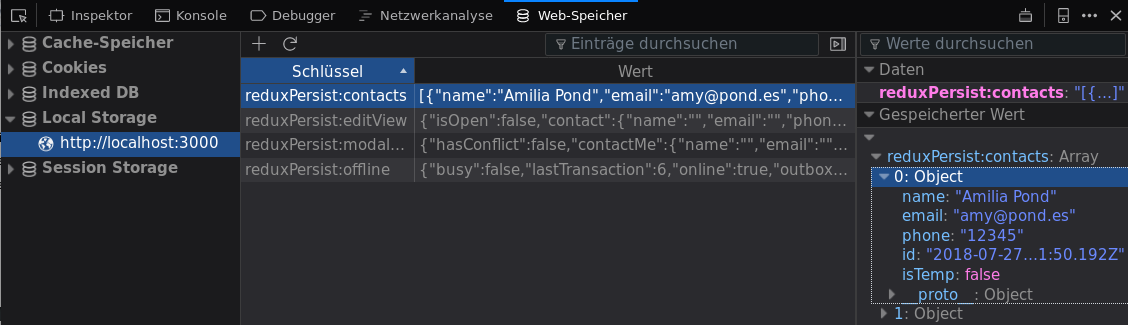
\includegraphics[width=\textwidth]{impl/localRdx}
  \grayRule
  \caption[Gespeicherte Daten im LocalStorage]{Gespeicherte Daten des Prototypen \it{amilia-rdx} im LocalStorage,\\Screenhot: Developer Tools im Firefox Browser}
  \label{fig:local-rdx}
\end{figure}
% 
Der Prototyp \it{amilia-qouch} nutzt zur lokalen Datenspeicherung PouchDB. PouchDB speichert die von NutzerInnen generierten Daten in IndexedDB, vgl. \autoref{chap:pouch}. In \autoref{fig:local-qouch} sind die gespeicherten Daten in der IndexedDB zu sehen.
%
\begin{figure}[H]
  \centering
  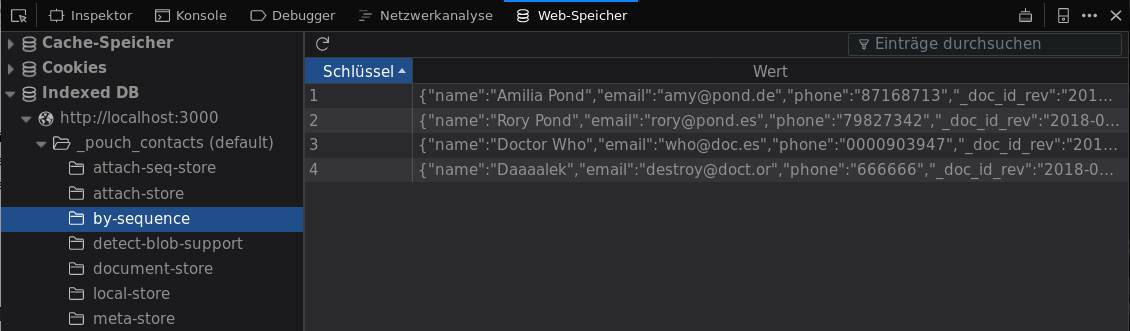
\includegraphics[width=\textwidth]{impl/localQouch}
  \grayRule
  \caption[Gespeicherte Daten in IndexedDB]{Gespeicherte Daten des Prototypen aus \it{amilia-qouch} in IndexedDB,\\Screenhot: Developer Tools im Firefox Browser}
  \label{fig:local-qouch}
\end{figure}
%
% SYNC
%
\sub{Datenbanksynchronisation}
Zwischen PouchDB und CouchDB können Daten in Echtzeit synchronisiert werden. Um die Live--Replikation zu aktivieren, muss im Synchronisationsaufruf der Parameter \tt{live: true} gesetzt sein.
Bricht die Internetverbindung ab, stoppt auch die Synchronisation.
Dank der angegebenen Parameter \tt{retry: true} versucht PouchDB die Synchronisation solange neuzustarten bis die Anwendung wieder mit dem Internet verbunden ist. \autoref{code:sync} zeigt die Implementation der Datenbankensynchronisation im Prototypen \it{amilia-qouch}.
%
\begin{center}
  \lstinputlisting[language=REACT,
  numbers=left,xleftmargin=20pt,
  firstline=1,lastline=5,
  framexleftmargin=15pt,
  caption={Synchronisation zwischen PouchDB und CouchDB im Prototyp \it{amilia-qouch}},
  label=code:sync]{code/sync.js}
\end{center}
Redux Offline nimmt einem auch Arbeit bei der Datensynchronisation ab. Alle Daten die sich im Queue befinden werden automatisch an den Server gesendet, sobald eine Internetverbindung besteht. Das funktioniert jedoch nicht so einfach wenn der Server nicht an ist. In der Dokumentation von Redux Offline steht, dass die Aktion solange versucht wird auszuführen, bis die Anwendung wieder mit dem Internet verbunden ist ~\cite{giving-up}. Allerdings wird die \sc{rollback} Aktion gefeuert wenn der Server nicht verfügbar ist und die Aktion wird abgebrochen.
\begin{center}
  \lstinputlisting[language=REACT,
  numbers=left,xleftmargin=20pt,
  firstline=6,
  framexleftmargin=15pt,
  caption={Discard Konfiguration für amilia-rdx},
  label=code:discard]{code/sync.js}
\end{center}
Die Discard Konfiguration bestimmt wann eine Aktion abgebrochen, und wann sie immer wieder neugestartet wird. Im \autoref{code:discard} ist in den Zeilen 1 bis 4 abzulesen wie diese Konfiguration überschrieben wird. Nun wird die Aktion nur abgebrochen wenn der Server verfügbar ist und einen \gls{HTTP} Status zwischen 400 und 500 zurückgibt.
In den darauffolgenden Zeilen wird die eigens implementierte Konfiguration mit der Standardkonfiguration von Redux Offline zusammengeführt wird.
Alle Daten werden nun auch nach einem Ausfall an den Server gesendet.\\
Im Gegensatz zum \it{amilia-qouch} Prototypen werden die Daten nur in eine Richtung automatisch gesendet. Es gibt keine Implementierung einer automatischen Replikation von den Daten auf dem Server zum lokalen Speicher.
%
%
%
\section{\label{chap:konfliktmanagement}Konfliktmanagement}
Konflikte werden in beiden Prototypen manuell erzeugt, wobei die Vorgehensweise identisch ist.
Wie ein Konflikt herbeigeführt werden kann, wird in \autoref{chap:konzept:test} beschrieben.
Durch das regelmäßige Anfragen an den Server wird ermittelt, ob sich die Anwendung im Onlinestatus befindet oder nicht.
Konflikte können erzeugt werden, wenn mindestens ein Gerät auf dem die Anwendung läuft, nicht mit dem Internet verbunden ist.
Die Anzeige des Netzwerkstatus im Header dient der Kontrolle über diesen Status.
Die folgenden Codeausschnitte illustrieren das Konfliktmanagement im Prototypen \it{amilia-qouch}.\\
Konflikte werden in CouchDB gespeichert, damit in der Anwendung entschieden werden kann wie damit umgegangen wird.
Im \autoref{code:conflicts} werden alle Kontakteinträge geladen.
Weil der Parameter in Zeile 3 als Option mitgegeben wird, sind Konfliktinformationen für jeden Kontakt verfügbar.
Gibt es unterschiedliche Versionen eines Kontaktes kommt er mit dem Attribut \tt{\_conflicts} beim Client an, und zwar in Form einer Liste aus allen korrelierenden Revisionsnummern.
In Zeile 7 wird der erste konfliktbehaftete Kontakt, der vom Server kommt, ermittelt.
Wenn es einen Konflikt gibt, wird die Funktion \tt{getConflictRevisions} in Zeile 10 aufgerufen.
%
\begin{center}
  \lstinputlisting[language=REACT,
    firstline=1,lastline=12,
    numbers=left,xleftmargin=20pt,framexleftmargin=15pt,
    caption={Das Laden von konfliktbehafteten Kontakten},
    label=code:conflicts]{code/conflicts.js}
\end{center}
%
\autoref{code:conflicts2} zeigt die Umsetzung der \tt{getConflictRevisions()}.
Hier wird die konkurrierende Version des Kontakts ermittelt.
Außerdem wird die Herkunft jeder Version festgestellt und das Öffnen eines Konfliktdialogs eingeleitet.\\
In Zeile 2 werden die Variablen \tt{contactMe} und \tt{contactYou} initialisiert.
Die erste repräsentiert die lokale Version, \tt{contactYou} steht für die Version die aus der CouchDB kommt.
In Zeile 4 wird überprüft, ob die übergebene Version des Kontakts mit der zuletzt bearbeiteten übereinstimmt.
Entsprechend werden die Variablen \tt{contactMe} und \tt{contactYou} befüllt.
Die übergebene Version ist die von CouchDB festgelegte gewinnende Revision.
Die andere, konkurrierende Version wird in Zeile 8, bzw. in Zeile 13 durch die Übergabe der Revisionsnummer im Parameter geladen.
Die ID ist bei beiden Versionen identisch.\\
%
Dann wird das Öffnen des Konfliktdialogs durch das Aktualisieren des \gls{App}status initialisiert.
Die beiden Kontaktversionen werden ebenfalls in den State geladen, um im Dialog korrekt angezeigt zu werden.
%
\begin{center}
  \lstinputlisting[language=REACT,
    firstline=14,lastline=38,
    numbers=left,xleftmargin=20pt,framexleftmargin=15pt,
    caption={Das Ermitteln von konkurrierenden Kontaktversionen},
    label=code:conflicts2]{code/conflicts.js}
\end{center}
%
Der Konfliktdialog ist in \autoref{fig:modal} dargestellt.
Im Titel steht der Name der lokalen Version, rot hervorgehoben.
Darunter befinden sich zwei große Knöpfe in unterschiedlichen Farben.
Der erste zeigt die Version des Kontakts, die vom Server kommt, die auf einem anderen Gerät bearbeitet wurde.
Der zweite, untere Knopf beinhaltet alle relevanten Informationen über die lokale Version des konfliktbehafteten Kontakts.
So ist zu erkennen welche der beiden Versionen die eigene ist und worin sie sich von der anderen unterscheidet.
%
\begin{figure}[H]
  \centering
  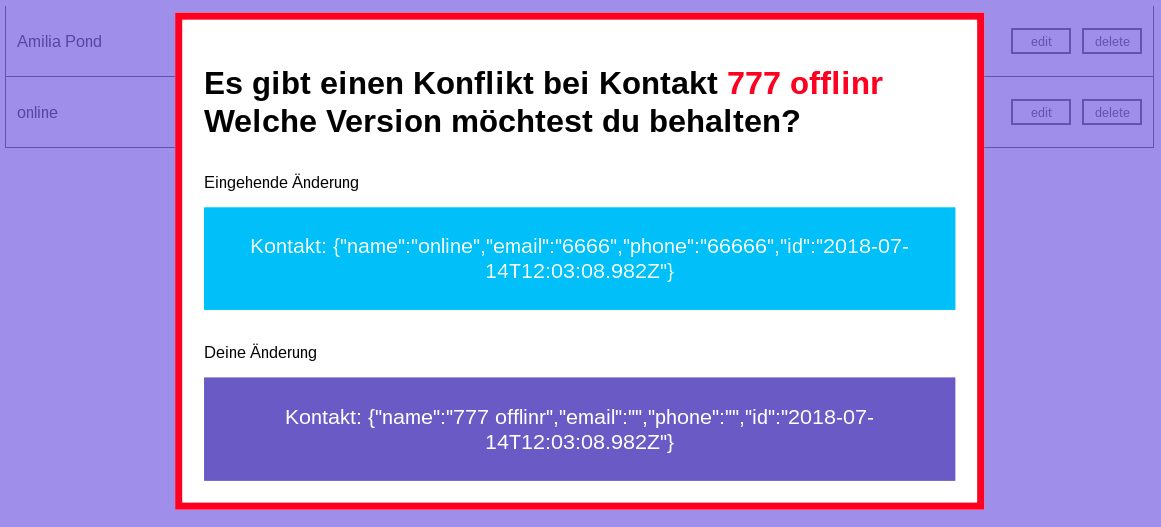
\includegraphics[width=\textwidth]{impl/Modal}
  \grayRule
  \caption{Konfliktdialog des Prototypen amilia-qouch}
  \label{fig:modal}
\end{figure}
%
Durch das Klicken einer dieser Knöpfe wird entschieden, welche der beiden Versionen behalten und welche eliminiert wird.
Wird der Knopf mit der lokalen Version betätigt, wird die in \autoref{code:conflicts3} gelistete Funktion \tt{removeRev} mit der anderen Version im Parameter aufgerufen.
%
\begin{center}
  \lstinputlisting[language=REACT,
    firstline=40,lastline=43,
    numbers=left,xleftmargin=20pt,framexleftmargin=15pt,
    caption={Das Eliminieren der verlierenden Version},
    label=code:conflicts3]{code/conflicts.js}
\end{center}
%
In Zeile 3 wird die verlierende Revision gelöscht.\\\\
%
%
Der Konfliktdialog konnte für den Protoypen \it{amilia-rdx} nicht umgesetzt werden, da Redux Offline nicht die Möglichkeit bietet Konflikte zu erkennen, geschweige denn zu speichern.
%
% Installationsanleitung
%
\section{Installationsanleitung}
\todo{build und so}
Beide entwickelten Prototypen sind als öffentliche Repositories auf GitHub\footnote{Software--Entwicklungs--Plattform \url{https://github.com/}} zu finden. 
Um sie zu installieren müssen folgende Schritte ausgeführt werden.
\sub{amilia-qouch}
1. Zuerst muss das Repository kopiert werden:
\lstset{language=sh, caption={},belowcaptionskip=0.3\baselineskip}
\begin{lstlisting}
git clone git@github.com:hulkoba/amilia-qouch.git
# oder
git clone https://github.com/hulkoba/amilia-qouch.git
\end{lstlisting}
2. Dann muss man in das Verzeichnis navigieren und alle Abhängigkeiten installieren.
\begin{lstlisting}
cd amilia-qouch
npm install
\end{lstlisting}
3. Mittels
\begin{lstlisting}
npm start
\end{lstlisting}
wird die Anwendung gestartet.
%
\sub{amilia-rdx}
1. Auch hier muss das Repository zuerst kopiert werden:
\lstset{language=sh, caption={},belowcaptionskip=0.3\baselineskip}
\begin{lstlisting}
git clone git@github.com:hulkoba/amilia-rdx.git
# oder
git clone https://github.com/hulkoba/amilia-rdx.git
\end{lstlisting}
2. Schritt zwei ist identisch mit dem in der \tt{amilia-qouch} Anleitung\\
3. Mittels
\begin{lstlisting}
npm run server
npm start
\end{lstlisting}
wird zuerst der Server, dann die Anwendung gestartet.

%
% Testfälle
%
\section{\label{chap:impl:test}Testfälle}
\section{\label{sec:impl:test}Testfälle}
Folgende Testfälle zur Offlinefunktionalität werden während der Entwicklung stetig durchgeführt. Das erfolgreiche Bestehen dieser Tests ist eine notwendige Qualitätseigenschaft der zu entwickelnden Prototypen.
\begin{description}[leftmargin=0.7cm,style=nextline]
\item[Netzwerkstatus:] 
Die Anwendung muss zu jeder Zeit den korrekten Netzwerkstatus anzeigen.\\
\item[Kontakte lesen:] 
Die Anwendung bei jedem Start die Kontakte aus dem lokalen Speicher oder aus der \it{Datenbank} laden.\\
\item[Kontakt anlegen:] 
Die Anwendung muss zu jedem Zeitpunkt in der Lage sein einen Kontakt mit jedem seiner Attribute anzulegen. Dazu muss er immer lokal gespeichert werden und sobald eine Internetverbindung besteht, persistiert werden.
Das Anlegen eines Kontakts im Offlinestatus ist für die Konfliktforcierung erforderlich.\\
\item[Kontakt bearbeiten:] 
Die Anwendung muss zu jedem Zeitpunkt in der Lage sein einen Kontakt mit jedem seiner Attribute zu bearbeiten. Ist keine Internetverbindung vorhanden, müssen die Änderungen lokal übernommen und später, sobald sich der Netzwerkstatus ändert, synchronisiert werden.
Das Bearbeiten eines Kontakts im Offlinestatus ist für die Konfliktforcierung erforderlich.\\
\item[Kontakt löschen:] 
Die Anwendung muss zu jedem Zeitpunkt in der Lage sein einen Kontakt zu löschen.
Das Löschen eines Kontakts im Offlinestatus ist für die Konfliktforcierung erforderlich.
\end{description}
\chapter{\label{chap:evaluation}Evaluation}
\section{Test}
\sub{Implementierungsaufwand}
Kann ja nicht wirklich getestet werden, würde ich nur in die Auswertung schreiben.
\sub{Offlinefunktionalität}
Offlinefunktionalität wurde stetig getestet, siehe \ref{sec:impl:test}
\sub{Konfliktmanagement}
\subsub{Tests mit 1 Gerät / Browser}
(um Redux Offline eine Chance zu geben...)
\subsub{Tests mit 2 Geräten / Browser}
Kontakt anlegen:
\begin{itemize}
	\item online -- online
	\item offline -- online
	\item offline -- offline
	\item trennen zwischen selben Feldern oder immer nur selbes Attribut bearbeiten?
\end{itemize}
Dasselbe für bearbeiten, löschen,
anlegen und bearbeiten, barbeiten und löschen, anlegen und löschen\\

%
% Auswertung
%
\section{Auswertung}
\sub{Implementierungsaufwand}
\begin{description}[leftmargin=0.7cm,style=nextline]
\item[Setup der App:] 
Irrelevant und identisch wegen Create React App.\\
\item[Einbinding der Technologien:] 
\b{PouchDB und CouchDB:} gering, nur Installation und Anwendung der Pouch API\\
Neue Instanz, Synchronisation ( 1 Zeile) und CRUD\\\\
\b{Redux Offline:} komplex, da Redux eingesetzt und verstanden werden muss. Für komplexere Apps mag das generell besser sein, aber für den einfachen Anwendungsfall zu viel Overhead. Einbindung von Redux Offline war allerdings wenig aufwändig sobald Redux implementiert war.\\
\item[Lesbarkeit des Codes:] 
\b{PouchDB und CouchDB:} nicht mehr als erwartet und auch verständlich wenn man mit den Technologien nicht vertraut ist. Es liest sich so wie man es verwendet dank unmissverständlicher API.\\\\
\b{Redux Offline:} Auch um den Code ohne Probleme lesen zu können muss man mit Redux vertraut sein. Ist das der Fall, ist trotzdem ein Blick in die Dokumentation von Redux Offline hilfreich, weil die Metaattribute nicht für sich selbst sprechen (effect, commit, rollback).\\
\end{description}
%
\sub{Offlinefunktionalität}
%
\sub{Konfliktmanagement}

%
\section*{Vergleich}
\begin{longtable}[c]{@{}
	>{\columncolor[HTML]{CFFCC2}}l ll@{}}
	\toprule
	\multicolumn{1}{p{0.1\textwidth}}{\cellcolor[HTML]{cffcc2}{}} 
  &
	\multicolumn{1}{p{0.45\textwidth}}{\cellcolor[HTML]{cffcc2}\textbf{PouchDB}}
	&
  \multicolumn{1}{p{0.45\textwidth}}{\cellcolor[HTML]{cffcc2}\textbf{Redux Offline}} \\
	
  \hline \noalign{\vskip 0.1cm}
	\endfirsthead
	\endhead
	%
\multicolumn{1}{p{0.1\textwidth}}
{\textbf{Storage}}
&       
\multicolumn{1}{p{0.45\textwidth}}
{IndexedDB WebSQL}
&                                                                                         
\multicolumn{1}{p{0.45\textwidth}}
{(redux-persist) Brwoser: IndexedDB oder WebSQL / LocalStorage, Fallbacks via localForage.
ReactNative: AsyncStorage}\\
\midrule
% ----------------------------------------------
\multicolumn{1}{p{0.1\textwidth}}
{\textbf{Requirements}}
&       
\multicolumn{1}{p{0.45\textwidth}}
{--}
&                                                                                         
\multicolumn{1}{p{0.45\textwidth}}
{Redux}\\
\midrule
% ----------------------------------------------
\multicolumn{1}{p{0.1\textwidth}}
{\textbf{Lines of Code}}
&       
\multicolumn{1}{p{0.45\textwidth}}
{?}
&                                                                                         
\multicolumn{1}{p{0.45\textwidth}}
{?}\\
\midrule

	%
	% end
	\bottomrule \cellcolor[HTML]{FFFFFF}
	\vspace{0.1cm}\\
	\noalign{\hspace{0.0525\textwidth}\grayRule}
	\caption{Anforderungen aus Entwicklungsperspektive}
	\label{tab:evaluation}\\
\end{longtable}

\chapter{\label{chap:fazit}Zusammenfassung und Ausblick}
Das System ist bei Bedarf auf verschiedene Weisen erweiterbar...

%
%	APPENDICES
%

%% Ein kleiner Abstand zu den Kapiteln im Inhaltsverzeichnis (toc)
\addtocontents{toc}{\protect\vspace*{\baselineskip}}


\printglossary[type=\acronymtype, title=Abkürzungen, style=super]
\printglossary[type=main,style=altlist]

%
%Abbildungsverzeichnis
%
\clearpage
\addcontentsline{toc}{chapter}{Abbildungsverzeichnis}
\listoffigures

% \renewcommand\lstlistlistingname{Quellcodeverzeichnis}
%\lstlistoflistings%quellcodeverzeichnis

%
% Literaturverzeichnis
%
\addcontentsline{toc}{chapter}{Literaturverzeichnis}
\bibliographystyle{alphadin}
\bibliography{appendices/literatur}
%
% Anhang
%
\clearpage
\appendix
\addcontentsline{toc}{chapter}{Anhang}
\chapter*{Anhang}
\section*{Eidesstattliche Erklärung}
\section*{CD-Inhalt}
Auf der beigefügten CD befinden sich
\begin{itemize}
	\item Die schriftliche Ausarbeitung dieser Masterrarbeit im PDF-Format
	\item Das erstellte Projekt
\end{itemize}

\end{document}
